\chapter{Apache Kafka in caso d’uso simulato}

\section{Definizione di un \textit{way of working}}

% Descrizione del Piano di Lavoro presentato, le strategie e il metodo di lavoro stabilito.
All'inizio del percorso ho delineato un \textit{way of working}, ovvero un metodo di lavoro da mantenere per tutta la durata dello \textit{stage}, insieme al tutor aziendale, il responsabile dell'area \sacr{eai} e gli esperti del settore.

Per garantire un buon livello organizzativo, quantificare l'avanzamento e rendere agevole la verifica e il supporto tecnico l'azienda ha proposto l'utilizzo di una \textit{board} di progetto.
Tra le tante opzioni disponibili, mi è stata proposta la piattaforma \textit{ClickUp}.
Rispetto alla concorrenza questa \textit{board} è ricca di funzionalità, pulita nell'esposizione dello stato del progetto, e la maggior parte delle sue funzioni sono gratuite.

All'inizio del percorso il tutor aziendale e il responsabile del \sacr{eai} hanno creato delle \textit{card} contenenti le attività previste per ogni settimana (\textit{task}) al fine di fornire una struttura generale del progetto.
All'interno di questi \textit{task} vi sono i concetti chiave, attività previste e obiettivi settimanali che lo stagista è tenuto a seguire per garantire l'efficacia del prodotto finale.
Oltre a questi \textit{task} principali, ho potuto creare di \textit{task} ausiliari e dei \textit{subtask} per descrivere più adeguatamente l'attività in corso.

Ciascun \textit{task} contiene una colonna laterale dove ho mantenuto un \textit{log} di tutto ciò che è stato eseguito relativo al \textit{task} in questione, allo scopo di esplicitarne il progresso e rendere agevole un eventuale supporto dal tutor o l'evoluzione futura.

Ogni settimana è previsto un \textit{online meeting} per la verifica del progresso ove necessario, la risposta ad eventuali questioni sollevate, e spiegazioni riguardo lo sviluppo della settimana successiva.
Alcune di queste videoconferenze ha visto la partecipazione di altri esperti che mi hanno aiutato a comprendere meglio il caso d'uso da reingegnerizzare, riassumendo lo stato attuale del sistema d'integrazione per uno dei clienti con relativi \textit{file} utilizzati.

Per mantenere alto il livello di organizzazione, efficienza ed efficacia, all'inizio di ogni giornata lavorativa ho creato un breve piano giornaliero con successivo consuntivo a fine giornata.
Questo ha permesso al tutor di verificare rapidamente il corretto avanzamento del processo in corso e al sottoscritto di mantenere il \textit{focus} su di esso.

\section{Formazione}

Il processo di Formazione ha avuto un importante ruolo all'interno dello \textit{stage}, con una durata complessiva di circa quattro settimane.
La causa di questo lungo periodo di formazione è data dallo studio di diversi ambiti e concetti per me nuovi, in particolare il settore del \textit{\acrlong{eai}} e la tecnologia di Kafka.

\bigskip
\begin{figure}[h]
  \begin{center}
    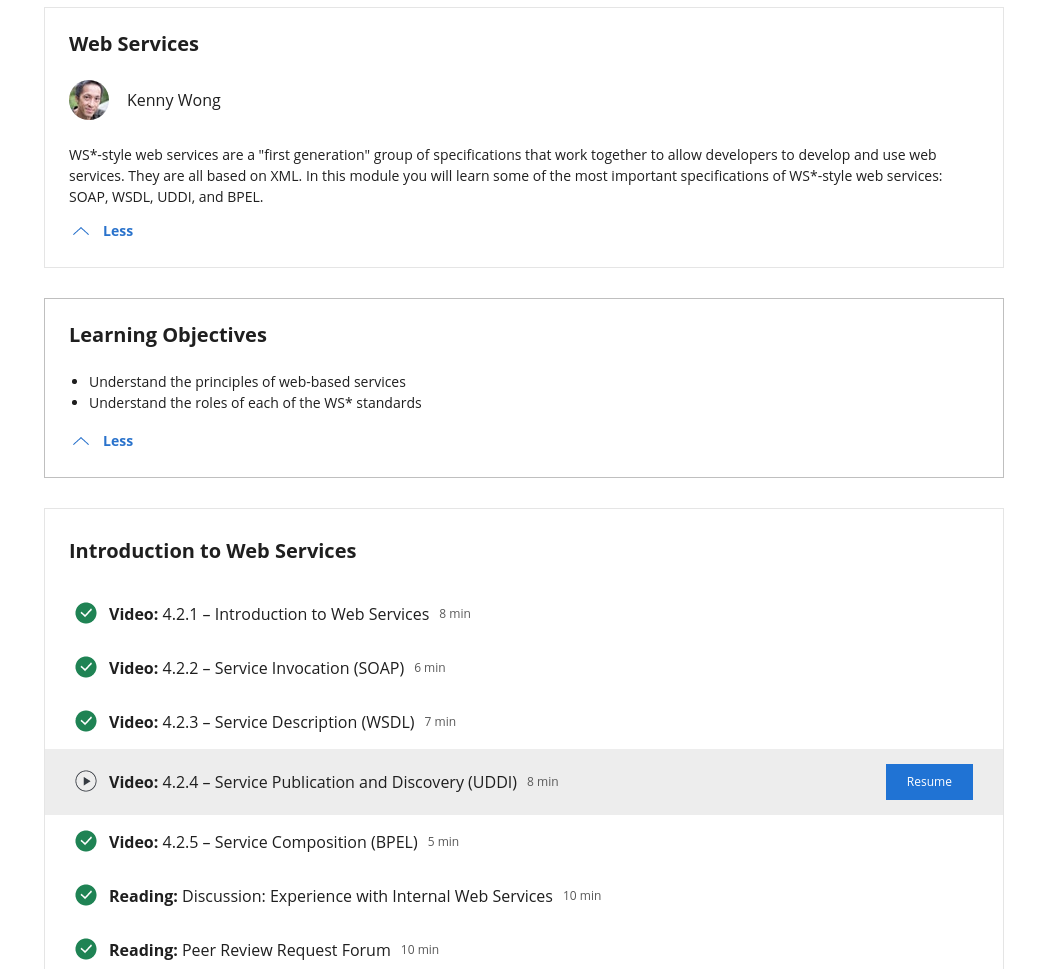
\includegraphics[width=0.7\textwidth]{images/coursera_week2.png}
    \caption{Screenshot del corso online \textit{acrlong{soa}} sulla piattaforma Coursera}
    \captionsetup{aboveskip=2pt}
    \caption*{\begin{footnotesize}\textit{Fonte: elaborazione personale}\end{footnotesize}}
  \end{center}
\end{figure}


Durante questo processo Sync Lab mi ha fornito del materiale didattico per l'apprendimento, quali diapositive e appunti di origine aziendale e l'accesso a dei corsi riguardo \textit{Software architecture}, \textit{\acrlong{soa}} (figura \thefigure) (tramite i corsi online su \textit{Coursera}) e Apache Kafka (tramite i corsi online su \textit{Udemy}).

Il tutor aziendale e responsabile \sacr{eai} hanno fornito durante i \textit{meeting} settimanali ulteriori chiarimenti e approfondimenti sul come Sync Lab applica questi concetti nello sviluppo di architetture \software.

Per i corsi online a maggiore contenuto nozionistico ho redatto degli appunti riassuntivi, con lo scopo di consolidare l'apprendimento e velocizzare la verifica del tutor aziendale.

\section{Analisi e progettazione di un caso d'uso}

Ad alcune videoconferenze ha partecipato anche un esperto \textit{senior} aziendale, esterno al progetto di \stage\ in questione, per illustrarmi un caso d'uso in cui l'azienda ha esposto un prototipo di sistema di integrazione utilizzando i concetti di \textit{Web Service}, \sacrfoot{soap} e \textit{request/response}, permettendomi la visualizzazione dei file \sacrfoot{wsdl}, \sacrfoot{xml} e \sacrfoot{xsd} associati.
Ho pertanto generato un caso d'uso adatto agli scopi dello \stage\ ispirandomi al caso d'uso reale illustrato.

Il caso d'uso modellato tratta una richiesta di credito telefonico da parte di un cliente ad un'azienda di telecomunicazioni tramite \textit{Web Service}, per soddisfare il requisito dello sviluppo della reingegnerizzazione del flusso di dati asincrono.
La \textit{request} avviene tramite flusso di un file \sacrfoot{json} che viene trasmesso attraverso i vari servizi che compongono il sistema di integrazione, basatosul \textit{Design Pattern} di tipo \textit{publish/subscribe}.

Va precisato che il contenuto di tale \sacr{json} non è strettamente rilevante allo sviluppo e funzionamento del \textit{Middleware}, ma aiuta a stabilire il contesto di utilizzo.

\bigskip
\begin{figure}[h]
  \begin{center}
    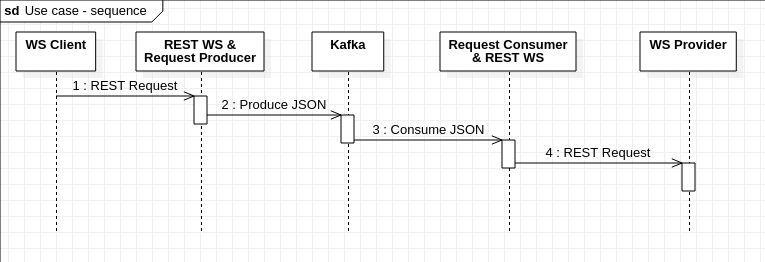
\includegraphics[width=\textwidth, trim={0.08cm 0 0 0.08cm},clip]{images/uc_sequence.png}
    \caption{Diagramma di sequenza \sacr{uml} per il prototipo di caso d'uso iniziale}
    \captionsetup{aboveskip=2pt}
    \caption*{\begin{footnotesize}\textit{Fonte: elaborazione personale}\end{footnotesize}}
  \end{center}
\end{figure}

\noindent
Il caso d'uso (figura \thefigure) è composto dai seguenti passaggi:
\begin{enumerate}
  \item il cliente (\textit{\sacrfoot{ws} Client}) effettua una richiesta di credito tramite invio di un file \sacr{json} al successivo Servizio Web in ascolto.
  \item il servizio composto da \sacrfoot{rest} \sacr{ws} e \textit{Request Producer} riceve il \sacr{json} e lo inserisce in Kafka tramite l'apposito \textit{Kafka Producer}, assumendo la funzione di \textit{publisher}.
  \item il servizio di \textit{Request Consumer}, sottoscritto al \textit{topic} in questione riceve il \sacr{json} e lo invia al \sacr{ws} finale tramite una \sacr{rest} request.
  \item il servizio in coda chiamato \sacr{ws} \textit{Provider} riceve il \sacr{json}; grazie ai dati ricevuti è in grado di fornire il servizio richiesto dal \textit{Client} nello \textit{step} 1.
\end{enumerate}

La modellazione dell'architetture e struttura del sistema da sviluppare seguirà questo prototipo di \sacrfoot{uc}.
Il modello associato al caso asincrono con \textit{callback} seguirà la stessa struttura e \textit{step} dello \sacr{uc} illustrato qui sopra, con l'aggiunta speculare del messaggio di ritorno.

\section{Progettazione architetturale}

La progettazione architetturale ha portato alla produzione di diversi diagrammi \sacr{uml} per rappresentare efficacemente l'architettura del prodotto e fornire un modello da seguire durante il processo di sviluppo.
Il processo ha richiesto frequenti \textit{meeting} e confronti per raggiungere un risultato finale soddisfacente al fine della sperimentazione.

La progettazione architetturale del prodotto comprende un \middleware\ centrale basato su di una \textit{acrlong{eda}} con l'utilizzo di Apache Kafka, e due componenti di \textit{testing} chiamati \textit{service client} e \textit{service provider}, che simulano due servizi esterni che comunicano con il middleware attraverso \sacr{rest} \textit{request}.

Il sistema è composto da molteplici microservizi, che comunicano attraverso la rete di Docker.
L'obiettivo della progettazione è modellare un \middleware\ che sia implementabile in una \textit{acrlong{soa}}, e consentirne la verifica e collaudo grazie ai servizi di \textit{testing}.

\begin{figure}[H]
  \begin{center}
    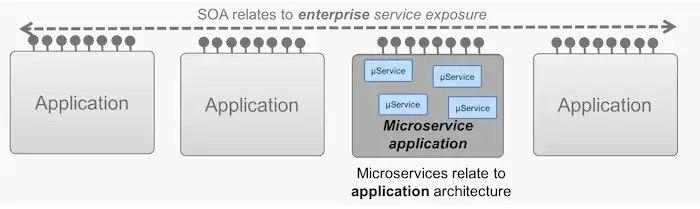
\includegraphics[width=0.7\textwidth]{images/soa_vs_micro.jpg}
    \caption{Visione ad alto livello delle differenze tra \sacr{soa} e microservizi}
    \captionsetup{aboveskip=2pt}
    \caption*{\begin{footnotesize}\textit{https://www.ibm.com/cloud/blog/soa-vs-microservices}\end{footnotesize}}
  \end{center}
\end{figure}

In figura \thefigure\ è rappresentata una visione ad alto livello dell'implementazione di un'applicazione a microservizi all'interno di una \sacr{soa}, evidenziando la differenza tra i due concetti.
\bigskip

Per rappresentare in modo chiaro ed elegante il modello descritto qui sopra, ho elaborato diversi diagrammi \sacr{uml}.
% I diagrammi di maggiore rilevanza, oltre ad essere esposti all'interno di questa sezione accanto alla spiegazione associata, sono allegati in formato più grande a
Questi diagrammi rappresentano i componenti \textit{color coded}, notazione utilizzata per dare continuità e chiarezza attraverso le diverse tipologie di \sacr{uml} \textit{diagrams}.

\subsubsection{\sacr{uml} \textit{sequence diagrams}}

\begin{figure}[H]
  \begin{center}
    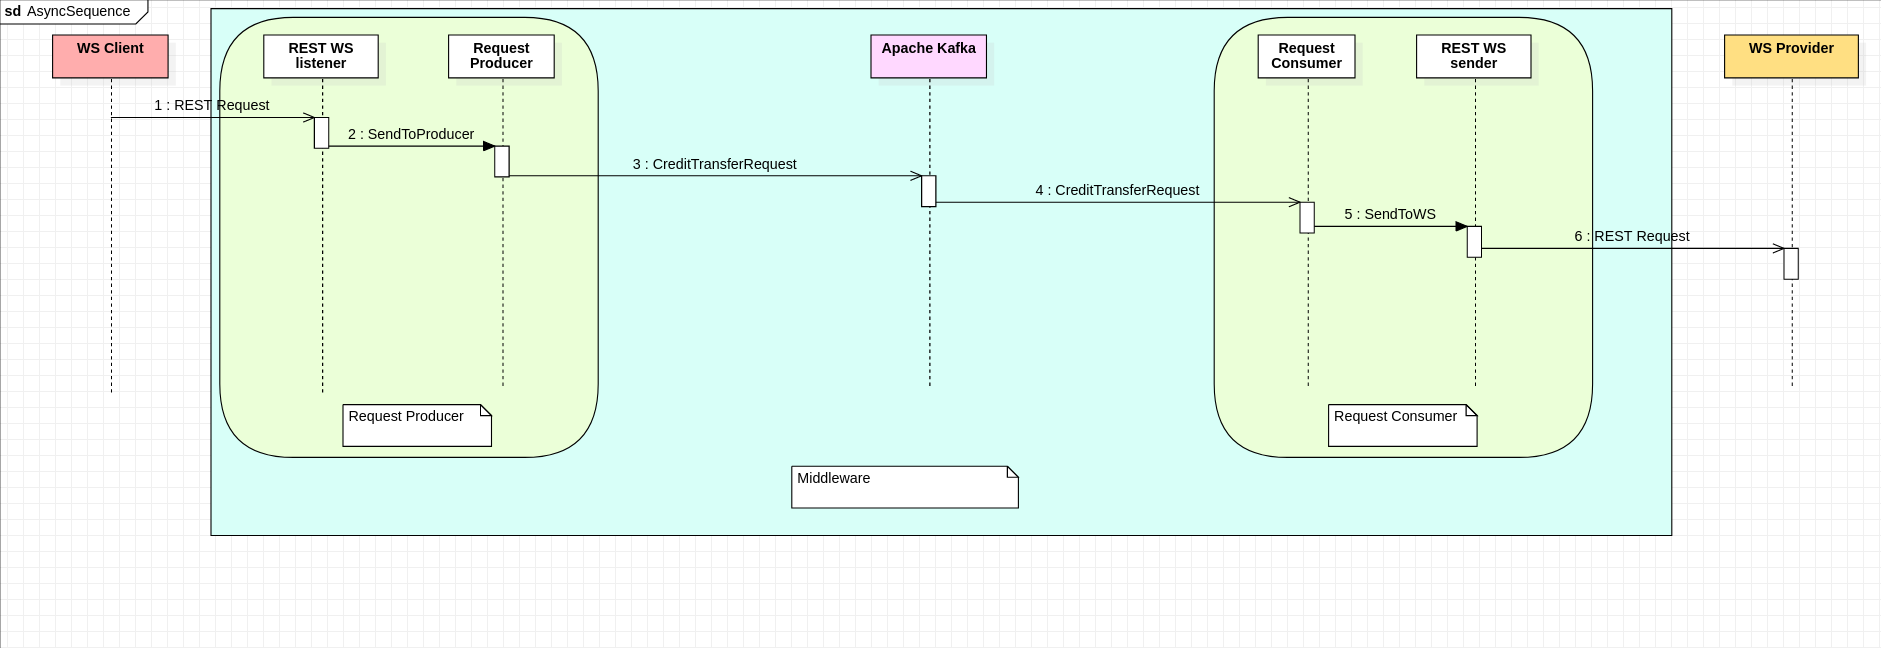
\includegraphics[width=\textwidth, trim={0.2cm 0 0 0.2cm},clip]{images/a_sequence2.png}
    \caption{Diagramma \sacr{uml} di sequenza per la reingegnerizzazione del flusso asincrono}
    \captionsetup{aboveskip=2pt}
    \caption*{\begin{footnotesize}\textit{Fonte: elaborazione personale}\end{footnotesize}}
  \end{center}
\end{figure}

A partire dallo \sacr{uc} descritto nela sezione precedente, ho prodotto un \sacr{uml} \textit{sequence diagram} più approfondito per rappresentare il flusso del \sacr{json} tra i vari componenti (figura \thefigure).

\begin{figure}[h]
  \begin{center}
    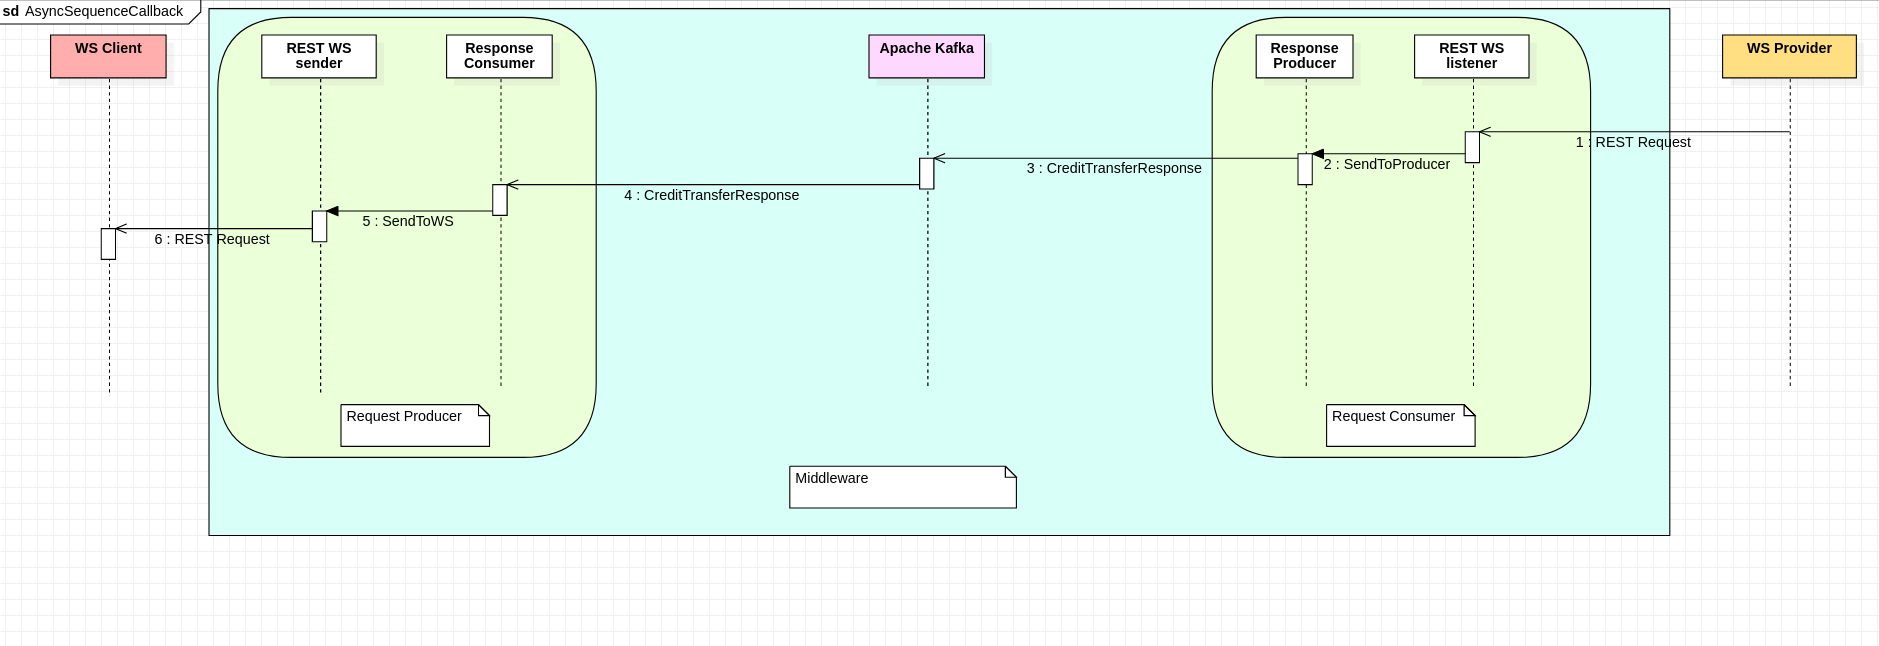
\includegraphics[width=\textwidth]{images/ac_sequence.png}
    \caption{Diagramma di sequenza \sacr{uml} per la reingegnerizzazione del flusso asincrono con \textit{callback}}
    \captionsetup{aboveskip=2pt}
    \caption*{\begin{footnotesize}\textit{Fonte: elaborazione personale}\end{footnotesize}}
  \end{center}
\end{figure}

La progettazione del sistema associato al caso asincrono con \textit{callback} comprende lo stesso schema \sacr{uml} del caso asincrono, con aggiunta del flusso di ritorno descritto nella figura \thefigure.

La reingegnerizzazione del flusso sincrono è stata scartata in favore dello studio di funzionalità aggiuntive tramite l'utilizzo della piattaforma di \textit{event streaming}.
La progettazione di un sistema basato su questo flusso era inizialmente prevista (come requisito desiderabile) nel piano di lavoro iniziale poiché associata ad un caso d'uso reale (di cui si è parlato nelle sezioni precedenti), ma infine è stata giudicata poco opportuna e fuori dagli scopi di Apache Kafka, un sistema basato sull'asincronicità

Il tempo associato a tale requisito è stato pertanto riproposto per testare un'altra funzione utile in un \middleware\, quali la trasformazione di alcuni dati presenti nel \sacr{json}.
Più precisamente, è stato aggiunto un dato sensibile che viene nascosto e sostituito con asterischi "*" dopo la produzione del \textit{topic} in Kafka grazie all'utilizzo di Kafka Streams.
\bigskip
\begin{figure}[h]
  \begin{center}
    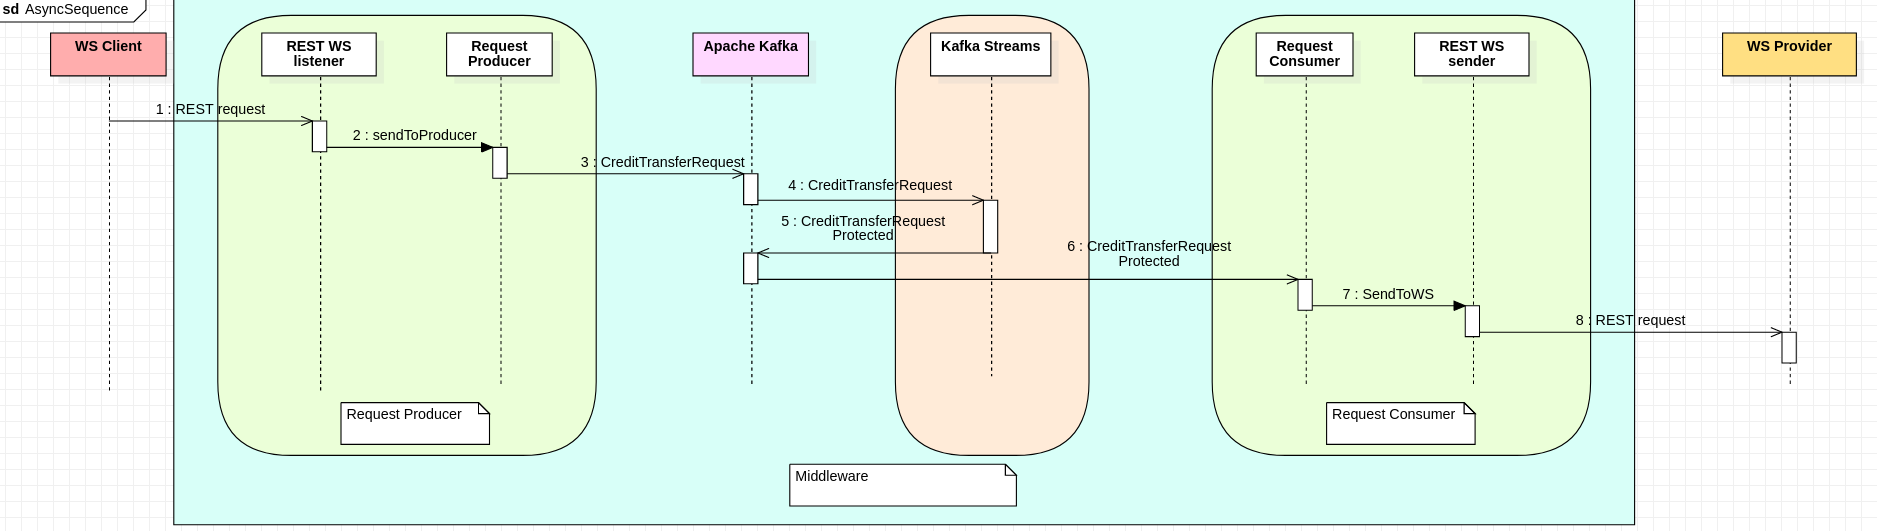
\includegraphics[width=\textwidth]{images/ap_sequence.png}
    \caption{Diagramma di sequenza \sacr{uml} per la reingegnerizzazione del flusso asincrono con protezione dei dati sensibili.}
    \captionsetup{aboveskip=2pt}
    \caption*{\begin{footnotesize}\textit{Fonte: elaborazione personale}\end{footnotesize}}
  \end{center}
\end{figure}

In figura \thefigure\ possiamo vedere il nuovo flusso asincrono con protezione (mascheramento) del dato sensibile.
La versione con \textit{callback} del flusso qui sopra prevede anche il flusso di ritorno (\textit{callback}), non illustrato in figura ma facilmente intuibile grazie al grafico che la precede.

\subsubsection{\sacr{uml} \textit{deployment diagrams}}

A supporto di questi \sacr{uml} \textit{sequence diagram} che rappresentano efficacemente il flusso di dati, punto focale dell'intero sistema di integrazione (asincrono con la protezione del dato sensibile), ho prodotto ulteriori diagrammi, tra i quali il \textit{deployment diagram}.
Questo diagramma ha lo scopo di rappresentare la configurazione dei processi \textit{run time}, modellando la struttura di base in cui eseguono i diversi servizi;
il diagramma esprime l'ambiente in cui i vari componenti risiedono e ove essi comunicano tra di loro.

Con l'approvazione degli esperti aziendali, ho deciso di appoggiare il sistema di integrazione sulla piattaforma Docker.

\begin{figure}[h]
  \begin{center}
    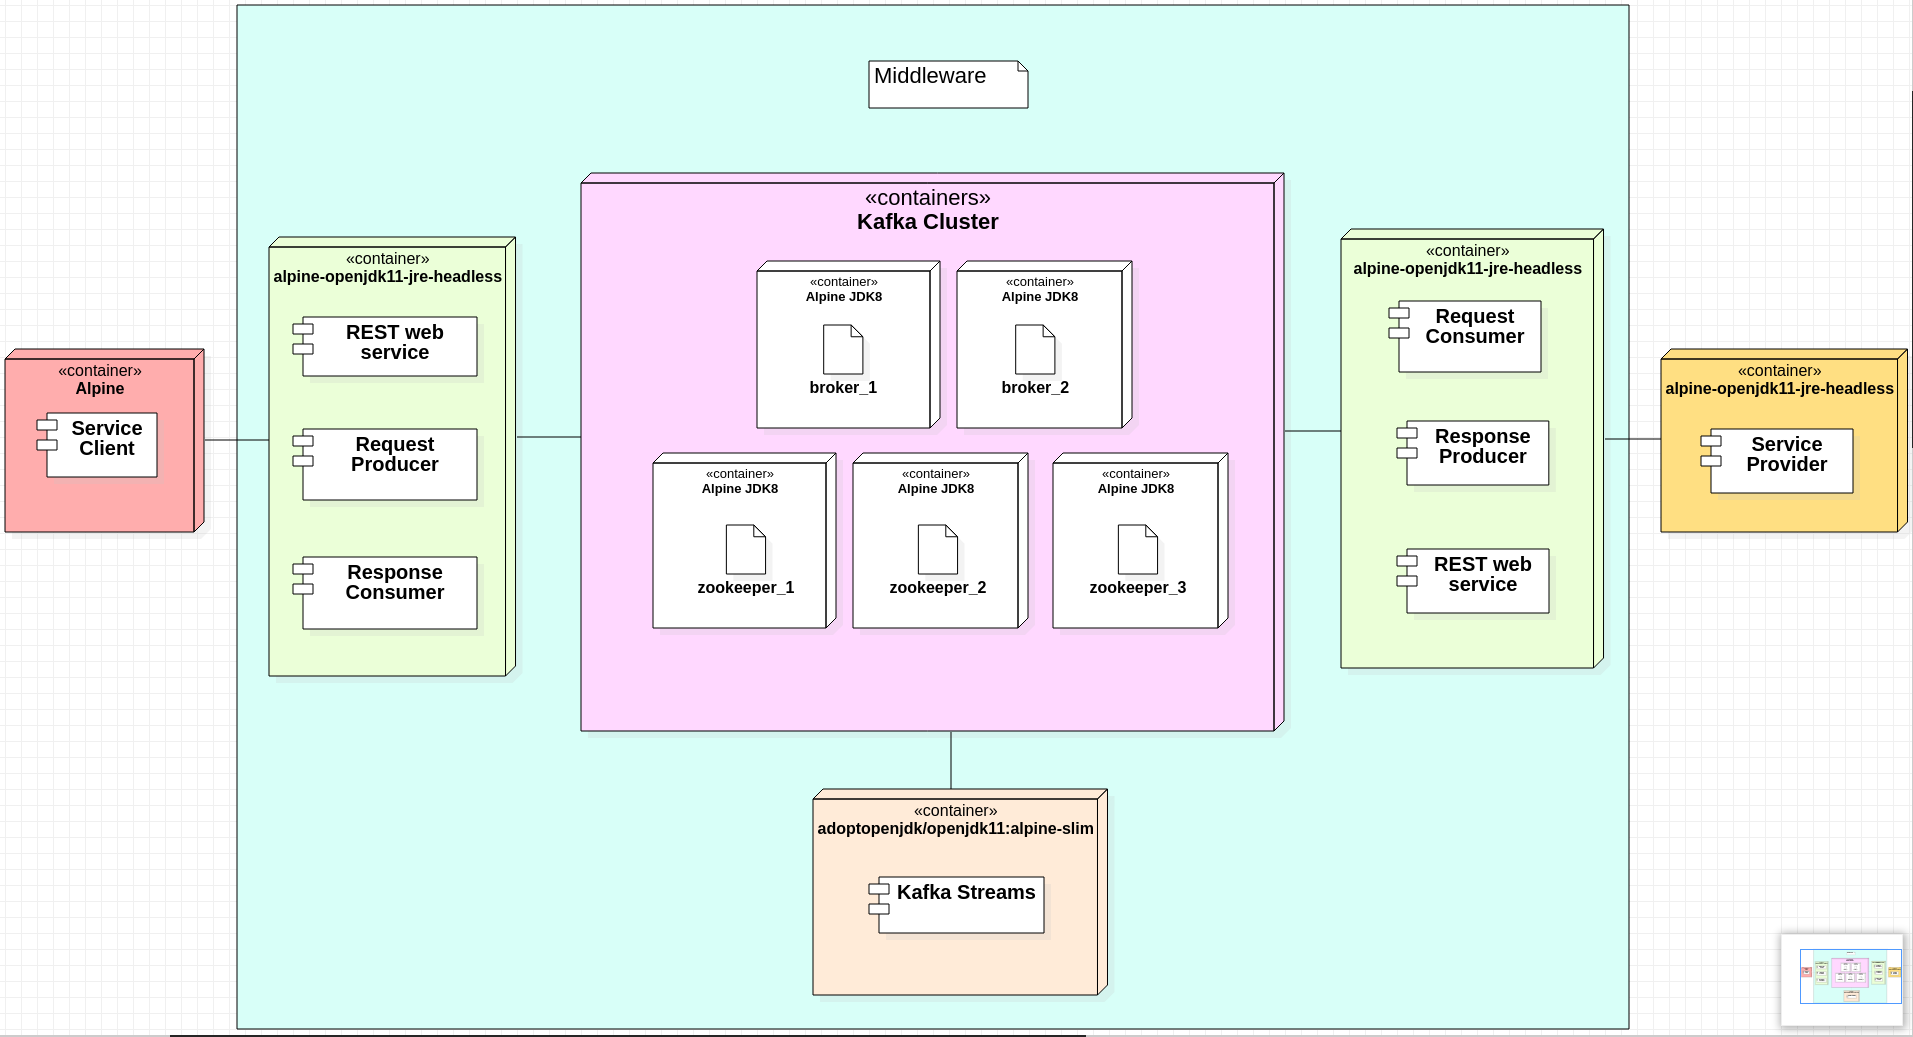
\includegraphics[width=\textwidth,  trim={0 0.2cm 0.2cm 0},clip]{images/ap_deployment.png}
    \caption{\sacr{uml} \textit{deployment diagram} per la reingegnerizzazione del flusso asincrono (protetto)}
    \captionsetup{aboveskip=2pt}
    \caption*{\begin{footnotesize}\textit{Fonte: elaborazione personale}\end{footnotesize}}
  \end{center}
\end{figure}

Il diagramma di \textit{deployment} (figura \thefigure) vede pertanto l'utilizzo di numerosi \textit{container} indipendenti che dialogano attraverso una rete locale all'interno di Docker.
Questi \textit{container} sono raffigurati dai vari nodi (rappresentati dai cubi in rilievo in figura).
A questa notazione fa eccezzione il nodo virtuale intitolato "Kafka Cluster", che ha solamente lo scopo di raggruppare i vari nodi legati al \textit{environment} di Kafka con funzione comune, ma che in realtà non compone un container reale a se stante.
All'interno di questi nodi sono rappresentati gli artefatti che eseguono nel relativo \textit{container}, per esplicitare la presenza dei componenti.
Si può inoltre notare che l'ambiente di Apache Kafka è composto da un \textit{cluster} composto da due servizi \textit{Broker} e tre servizi \textit{Zookeeper}, allo scopo di simulare un caso d'uso reale in cui i diversi componenti sono distribuiti in sistemi indipendenti e garantiscono l'affidabilità dello \textit{streaming} di eventi.

\subsubsection{\sacr{uml} \textit{component diagram}}

\begin{figure}[H]
  \begin{center}
    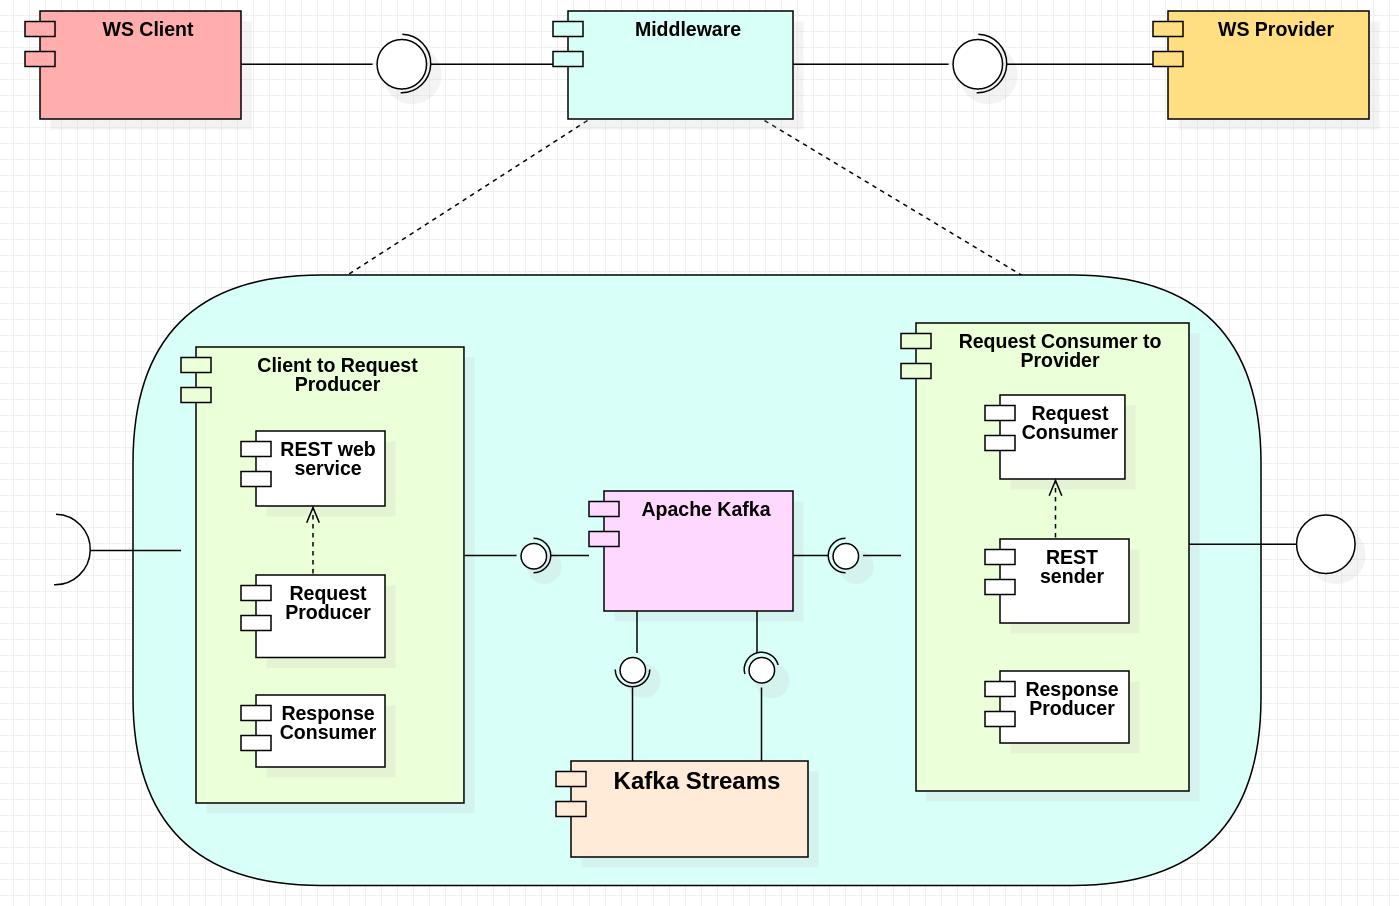
\includegraphics[width=\textwidth]{images/ap_component.png}
    \caption{\sacr{uml} \textit{component diagram} per la reingegnerizzazione del flusso asincrono (protetto)}
    \captionsetup{aboveskip=2pt}
    \caption*{\begin{footnotesize}\textit{Fonte: elaborazione personale}\end{footnotesize}}
  \end{center}
\end{figure}

Allo scopo di riassumere elegantemente i vari componenti del sistema ho elaborato un \sacr{uml} \textit{component diagram}.
Esso riassume con una visione ad alto livello i componenti che compongono il sistema e le modalità con cui esse interagiscono attraverso le relative interfacce.


% , basati su delle immagini Linux leggere e personalizzate.

% Come si può vedere dalla figura \thefigure,

% \section{\textit{Setup} dell'ambiente di lavoro}


\section{Sviluppo}

\subsection{Kafka \textit{cluster}}

Il primo passo del processo di sviluppo è stato quello del \textit{setup} dell'ambiente di Kafka in locale.
La guida rapida online fornita direttamente da Apache per un'installazione minimale di Kafka porta al \textit{download} di un pacchetto e l'esecuzione di un servizio Zookeeper e un \textit{broker} di Kafka.

Zookeeper è un servizio attualmente essenziale al funzionamento di Kafka, gestisce i nodi del \textit{cluster} e mantiene una lista dei topic e dei messaggi.
Le versioni future di Kafka renderanno questo servizio non necessario, ma attualmente sono ancora in fase di sviluppo e non adatta all'ambiente di produzione.
I due \textit{broker} si occupano di ricevere i messaggi dai \textit{producer}.

Dopo un breve collaudo del corretto funzionamento dei servizi tramite l'inserimento di un evento in un \textit{topic} e la relativa lettura, ho iniziato ad espandere e trasportare il sistema su dei \textit{container} Docker.

Il \textit{cluster} di Kafka utilizzato nel progetto di \stage\ è composto dai componenti descritti dalla progettazione architetturale nella sezione precedente, ovvero tre servizi di Zookeeper e due \textit{broker} per rappresetare un sistema di piccole dimensioni che tuttavia si avvicina ad un caso d'uso reale poichè contiene multipli Zookeeper e multipli \textit{broker}.

Questi cinque servizi necessitano dunque di eseguire contemporaneamente in un ambiente containerizzato con Docker connessi alla stessa \textit{network} locale, che consente ai diversi servizi di scambiare messaggi tra di essi.

Ho implementato questo \textit{cluster} tramite un
\textit{file} di tipo \texttt{yml} utilizzato dall'estensione Docker-compose.

\noindent
Il \textit{file} contiene una lista di servizi, in cui in ognuno viene specificato:
\begin{itemize}
  \item l'immagine Docker su cui viene costruito il servizio o il \texttt{dockerfile} da utilizzare per la sua costruzione;
  \item il nome del \textit{container};
  \item il nome del servizio;
  \item le dipendenze funzionali del servizio;
  \item l'indirizzo \sacr{ipv4} statico e le porte attraverso cui è possibile raggiungere il servizio all'interno della rete locale dagli altri \textit{container}.
\end{itemize}

\subsection{Kafka \textit{producer} e \textit{consumer}}

Il passo successivo è stato quello di sviluppare dei semplici \textit{producer} e \textit{consumer} in grado di inserire e leggere i dati in Kafka.
Una volta collaudati rapidamente questi due eseguibili scritti in Java, li ho incapsulati all'interno di un'applicazione utilizzando lo strumento di \textit{build} e gestione delle dipendenze Maven\footfullcite{maven}.

Per completare il modulo che costituisce il prototipo di \middleware\ è necessario che il \textit{producer} e \textit{consumer} siano in grado di comunicare con dei servizi esterni e fornire le interfacce adatte al ruolo.
Nel caso più complesso del flusso asincrono con \textit{callback}, entrambi questi servizi devono essere in grado di restare in ascolto di eventuali \sacr{rest} \textit{request} (che nel mio progetto utilizzano il protocollo \sacr{http}) e al tempo stesso di inviarle.

Ho pertanto creato un \sacr{http} \textit{server} minimale in Java attraverso il \textit{framework} Netty\footfullcite{netty}, in esecuzione in un \textit{thread} Java.
Sviluppi futuri vedrebbero probabilmente l'utilizzo di un \textit{framework} più evoluto come Spring Boot\footfullcite{spring}.
Un altro \textit{thread} si occupa invece dell'invio delle \sacr{rest} \textit{request} al servizio di destinazione, una volta ricevuto un evento da parte del \textit{consumer}.

\bigskip\noindent
L'insieme di questi componenti formano i blocchi logici illustrati in verde nella sezione precedente, in cui il primo servizio è formato da:
\begin{itemize}
  \item \sacr{rest} \textit{\acrlong{ws}} (\sacr{http} \textit{server} in ascolto);
  \item \textit{request producer};
  \item \textit{response consumer} (\textit{callback});
\end{itemize}
\noindent
e il secondo da:
\begin{itemize}
  \item \textit{request consumer};
  \item \sacr{rest} \textit{\acrlong{ws}} (invio della \textit{request});
  \item \textit{response producer} (\textit{callback}).
\end{itemize}

\subsection{\sacr{ws} \textit{Client} e \sacr{ws} \textit{Provider} }



\section{Collaudo}

Confronto con i requisiti posti nel piano di lavoro, valutazione riguardo i risultati raggiunti, quelli non raggiunti e i possibili sviluppi futuri
